\subsection{Logic.util-Quellpaket}
    \subsubsection{Logger}
        \begin{table}[H]
            \caption{Klasse Logger}
            \begin{tabular}{p{2.5cm}  p{9.5cm}} 
                \hline
                \textbf{Eigenschaft} & \textbf{Beschreibung}\\
                \hline
                Name & Logger\\
                Ort & Quellpaket \textit{logic.util}\\
                \hline
                Zweck &
                Die Klasse \textit{Logger} bietet die Möglichkeit Spielinformationen in einer Datei zu speichern 
                \\
                \hline
                Struktur &
                \begin{itemize}
                    \itemsep0em
                    \item Die \textit{printNewGame}-Methode speichert die generellen Informationen des Spielfeldes
                    \item Die \textit{printMove}-Methode speichert jeweils einen Zug eines Spielers
                \end{itemize}
                \\
                \hline
            \end{tabular}
        \end{table}
        \begin{figure}[H]
            \centering
            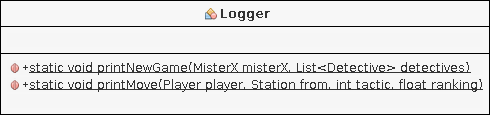
\includegraphics[scale=0.7]{img/uml/logger.png}   
            \caption{Logger UML-Klassendiagramm}
        \end{figure}


    \subsubsection{JsonValidator}
        \begin{table}[H]
            \caption{Klasse JsonValidator}
            \begin{tabular}{p{2.5cm}  p{9.5cm}} 
                \hline
                \textbf{Eigenschaft} & \textbf{Beschreibung}\\
                \hline
                Name & JsonValidator\\
                Ort & Quellpaket \textit{logic.util}\\
                \hline
                Zweck &
                Bietet Methoden zur Überprüfung der \textit{JSON}-Datenstruktur für einen Spielstand und des Netzes.
                \\
                \hline
                Struktur &
                \begin{itemize}
                    \itemsep0em
                    \item Die \textit{validateBoard}-Methode validiert die \textit{JSON}-Datenstruktur des Spielfeldes
                    \item Die \textit{validateSaveState}-Methode validiert die \textit{JSON}-Datenstruktur der Spielstandsdatei
                \end{itemize}
                \\
                \hline
            \end{tabular}
        \end{table}
        \begin{figure}[H]
            \centering
            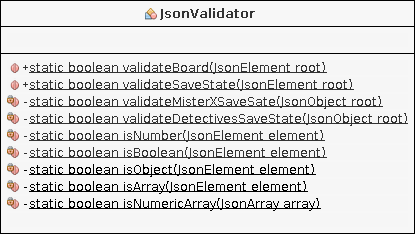
\includegraphics[scale=0.7]{img/uml/jsonValidator.png}   
            \caption{JsonValidator UML-Klassendiagramm}
        \end{figure}

    \subsubsection{GameLogicSerializer}
        \begin{table}[H]
            \caption{Klasse GameLogicSerializer}
            \begin{tabular}{p{2.5cm}  p{9.5cm}} 
                \hline
                \textbf{Eigenschaft} & \textbf{Beschreibung}\\
                \hline
                Name & GameLogicSerializer\\
                Ort & Quellpaket \textit{logic.util}\\
                \hline
                Zweck &
                Die \textit{GameLogicSerializer}-Klasse ist eine Hilfsmethode für die \textit{GSON}-Bibliothek
                und bietet einen benutzerdefinierten Serialisierer für die \textit{GameLogic}.
                \\
                \hline
                Struktur &
                \begin{itemize}
                    \itemsep0em
                    \item Wird von \textit{GSON} selbst instanziiert und verwendet.
                    Bietet über die \textit{serialize}-Methode die Möglichkeit eine \textit{GameLogic}-Instanz in ein \textit{JsonObject}
                    nach Aufgabenstellung zu transformieren.
                \end{itemize}
                \\
                \hline
            \end{tabular}
        \end{table}
        \begin{figure}[H]
            \centering
            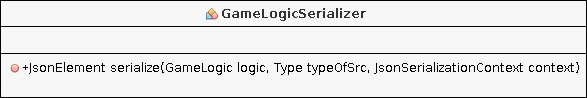
\includegraphics[scale=0.6]{img/uml/gameLogicSerializer.png}   
            \caption{GameLogicSerializer UML-Klassendiagramm}
        \end{figure}

    \subsubsection{MisterXSerializer}
        \begin{table}[H]
            \caption{Klasse MisterXSerializer}
            \begin{tabular}{p{2.5cm}  p{9.5cm}} 
                \hline
                \textbf{Eigenschaft} & \textbf{Beschreibung}\\
                \hline
                Name & MisterXSerializer\\
                Ort & Quellpaket \textit{logic.util}\\
                \hline
                Zweck &
                Die \textit{MisterXSerializer}-Klasse ist eine Hilfsmethode für die \textit{GSON}-Bibliothek
                und bietet einen benutzerdefinierten Serialisierer für \textit{MisterX}.
                \\
                \hline
                Struktur &
                \begin{itemize}
                    \itemsep0em
                    \item Wird von \textit{GSON} selbst instanziiert und verwendet.
                    Bietet über die \textit{serialize}-Methode die Möglichkeit eine \textit{MisterX}-Instanz in ein \textit{JsonObject}
                    nach Aufgabenstellung zu transformieren.
                \end{itemize}
                \\
                \hline
            \end{tabular}
        \end{table}
        \begin{figure}[H]
            \centering
            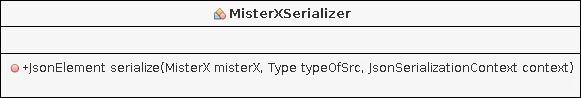
\includegraphics[scale=0.6]{img/uml/misterXSerializer.png}   
            \caption{MisterXSerializer UML-Klassendiagramm}
        \end{figure}


    \subsubsection{DetectiveSerializer}
        \begin{table}[H]
            \caption{Klasse MisterXSerializer}
            \begin{tabular}{p{2.5cm}  p{9.5cm}} 
                \hline
                \textbf{Eigenschaft} & \textbf{Beschreibung}\\
                \hline
                Name & MisterXSerializer\\
                Ort & Quellpaket \textit{logic.util}\\
                \hline
                Zweck &
                Die \textit{DetectiveSerializer}-Klasse ist eine Hilfsmethode für die \textit{GSON}-Bibliothek
                und bietet einen benutzerdefinierten Serialisierer für \textit{Detective}.
                \\
                \hline
                Struktur &
                \begin{itemize}
                    \itemsep0em
                    \item Wird von \textit{GSON} selbst instanziiert und verwendet.
                    Bietet über die \textit{serialize}-Methode die Möglichkeit eine \textit{Detective}-Instanz in ein \textit{JsonObject}
                    nach Aufgabenstellung zu transformieren.
                \end{itemize}
                \\
                \hline
            \end{tabular}
        \end{table}
        \begin{figure}[H]
            \centering
            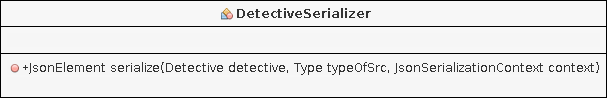
\includegraphics[scale=0.6]{img/uml/detectiveSerializer.png}   
            \caption{DetectiveSerializer UML-Klassendiagramm}
        \end{figure}

